\section{Data provided and method}
\protect\label{section:tdataprovided}

\subsection{Data Available}

The following data is available from the Red Dots project site:

\begin{itemize}
  \item Images taken with visible light filters \textbf{g},
\textbf{i}, \textbf{r} and \textbf{z} taken almost daily.
\item Flat file images taken almost every day, usually as 3 images from the sky,
taken as the light fades.
\item Bias file images taken each day (approximately 8 hours after the
observations).)
\item Monthly master flat file images for each month constructed from some of
the daily flat files.
\item Monthly master bias file images for each month, constructed from some of
the daily bias files.
\item REMIR infrared images taken almost every day up to June 2019.
\end{itemize}

The flat and bias images are only available for the visible light filters \textbf{g},
\textbf{i}, \textbf{r} and \textbf{z}.
Images, flat and bias files for the visible light filters are all taken at
exactly the same time for each of the four filters.

The REMIR infrared images, from the three filters \textbf{H}, \textbf{J} and
\textbf{K}. are divided approximately equally between 7 dither patterns. They
are only 512x512 pixels in size and no flat or bias files are provided. They are
not considered in this report. In any case they were discontinued at the start
of June 2019.

The total number of all observations as of \date{\today} is given in Table
\ref{table:tobbsnums} and the number of observations of each target is given in
Table \ref{table:tobbsnums}, the left panel includes the infrared images and the
right excludes these. The distribution of observations for the 3 main targets by date are shown in
Fig. \ref{fig:targobsplot}.

\begin{table}[!htbp]
\centering
\begin{tabular}{lr} \hline
  Filter & Number\\\hline
g & 39,922 \\
i & 39,921 \\
r & 39,916 \\
z & 58,268 \\
H & 36,854 \\
J & 50,574 \\
K & 34,683 \\
GRISM & 16,959 \\

\hline
\end{tabular}
\caption{This shows the total number of observations taken as of \date{\today},
both for visible light filters \textbf{g},
\textbf{i}, \textbf{r} and \textbf{z} and also for infrared filters \textbf{H}, \textbf{J} and
\textbf{K}. Note that infrared observations ceased at the beginning of June
2019.} \protect\label{table:tobbsnums}
\end{table}

\begin{table}[!htbp]
\begin{minipage}{.5\linewidth}
\centering
\begin{tabular}{lrr} \hline
  Target & Number & \%age\\\hline
\bstar & 17,592 & 5.71 \\
Ross 154 & 43,023 & 13.96 \\
\prox & 58,090 & 18.85 \\
Others & 189,531 & 61.49 \\
\hline
Total & 308,236 \\

\hline
\end{tabular}
\end{minipage}
\begin{minipage}{.5\linewidth}
\centering
\begin{tabular}{lrr} \hline
Filter & Number & \%age\\\hline
\bstar & 7,229 & 4.98 \\
P525-E & 7,404 & 5.10 \\
Ross 154 & 16,196 & 11.15 \\
\prox & 23,996 & 16.51 \\
Others & 90,475 & 62.27 \\
\hline
Total & 145,300 \\

\hline
\end{tabular}
\end{minipage}
\caption{Left panel is a list of observation targets and totals of all
observations taken as of \date{\today} including the infrared filters. The right
panel is the same, also of \date{\today}, for just the visible list filters.}.
\protect\label{table:obstargets} \protect\label{table:filtersnums}
\end{table}


\begin{figure}[!htbp]
\begin{center}
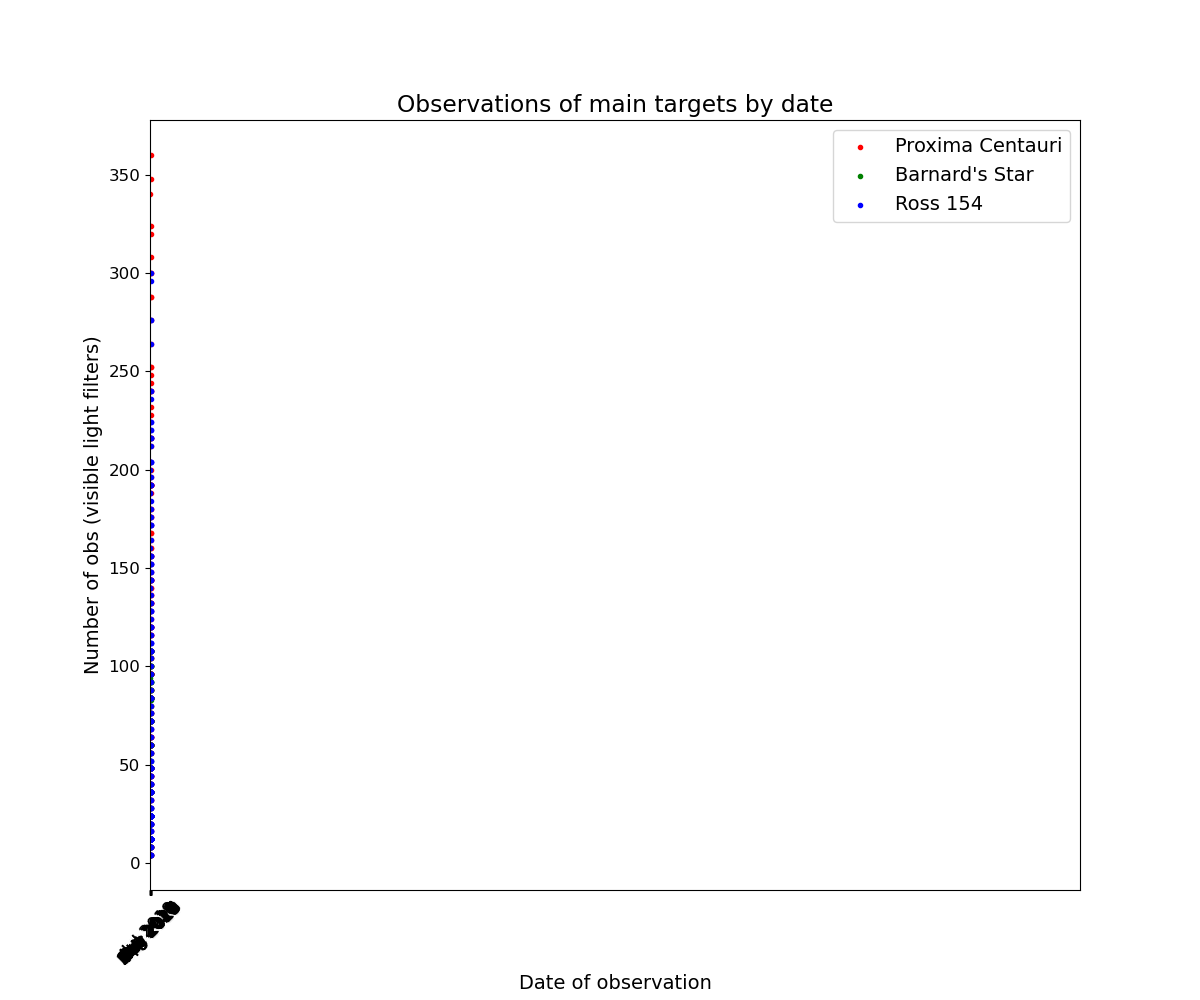
\includegraphics[scale=0.5]{images/visobstot.png} \\
\end{center}   
\caption{This figure shows the observations of the 3 target stars by date, as
of \date{\today}.}
\protect\label{fig:targobsplot}
\end{figure}
\subsection{Database and tools}
\protect\label{section:database}

To aid in the analysis of the data, a database was created using MySQL to
record and provide for fast retrieval of the observational data, flat file
images and results, together with software tools and library routines in Python
and Perl.

The images were processed according to the formula:

\begin{center}
$ \frac{(mage - bias) \times mf}{flat - bias}$
\end{center}

In this $mf$ represents to mean value of the flat pixels. The master flat files
provided already have the bias subtracted.

Half of the daily flat and bias files were made with a gain of 4.4, in line with
observations taken of targets other than the 3 main {\rdwarf} targets. As these
latter targets were all observed with a gain of 1, only the daily flat and bias
files with a gain of 1 were considered. The master bias files are
constructed from the daily bias files with a gain of 1. Accordingly attention is
restricted to images with a gain of 1.

\subsection{Attempts to display files}

All the standard display tools and routines struggled to show images with any
degree of contrast. Finding objects in images proved difficult also. The
best results were found from the images for \texttt{g} filter, followed by
those for the \texttt{r} filter. The images from the \texttt{i} and \texttt{z}
filters proved particularly hard to both display and hard to automatically find
objects within the images and not be confused by ``hotspots'' on the CCD.

In figure \ref{fig:exampmontage} is shown a sample from a fruitful viewing
night, 17th October 2019, showing images taken at the same time for each the
visible light filters, It is noticeable how with the \texttt{g} filter 10 objects
were found, with the \texttt{r} filter 3 objects were found, with the \texttt{i}
filter 2 objects and with the \texttt{z} filter, 1 object was found. (These
totals include the target, in this instance \bstar, in each case).

\begin{figure}[!htbp]
\begin{center}
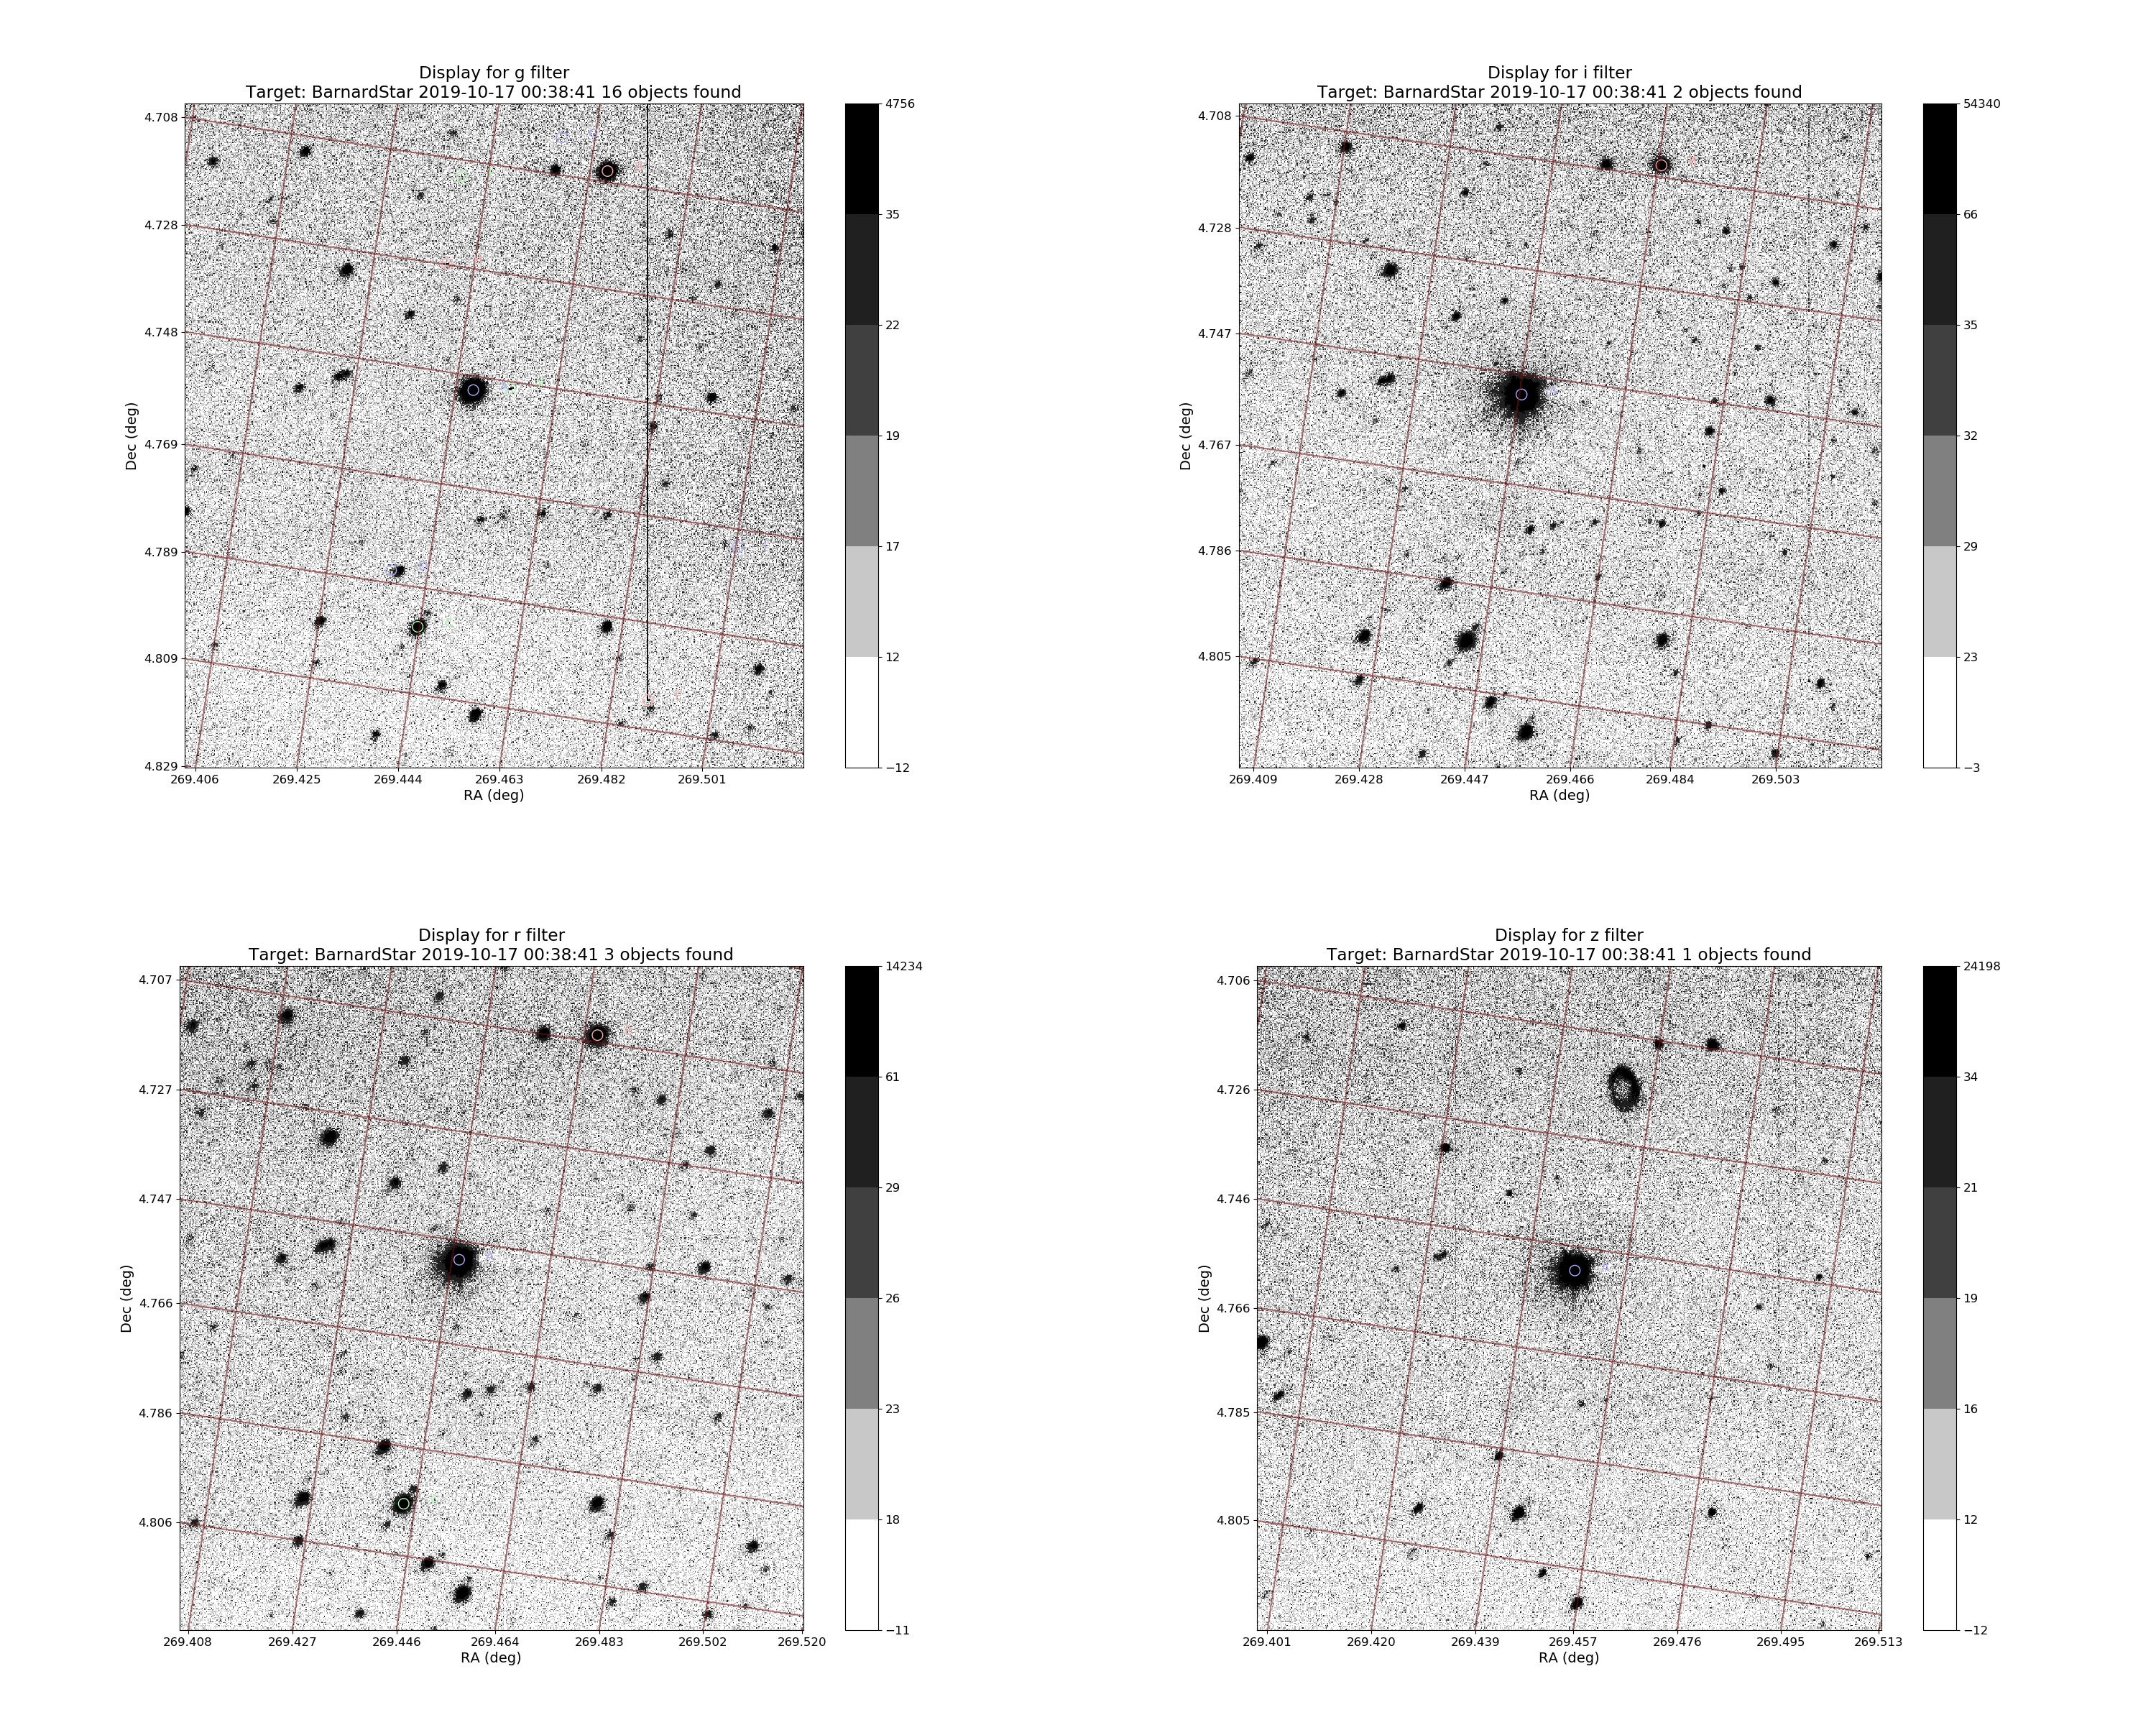
\includegraphics[scale=0.125]{images/exampmontage.png} \\
\end{center}   
\caption{In this figure is shown the same patch of sky as seen by each of the
four visible light filters at exactly the same time on 17th October 2019, with
\texttt{g} at the top left, \texttt{i} at the top right, \texttt{r} at the bottom left and \texttt{z} at the bottom right.
The master flat and bias for October 2019 for the appropriate filters was used.
Objects are marked with A, B, C etc to show
the objects found in descending order of ADU count. No attempt is
made here to identify the objects or optimise the aperture beyond a circular radius of 6 pixels,
however the brightest object (marked 'A') is \bstar.
The vertical line 2/3 of the way across and 3/4 of the way down the image for
the  \texttt{g} appears to be an artefact of column 623 of the CCDs.} 
\protect\label{fig:exampmontage}
\end{figure}

It is noteworthy that the same area of sky is rarely selected on consecutive
nights as is illustrated in Fig. \ref{fig:yearapart}.

\begin{figure}[!htbp]
\begin{center}
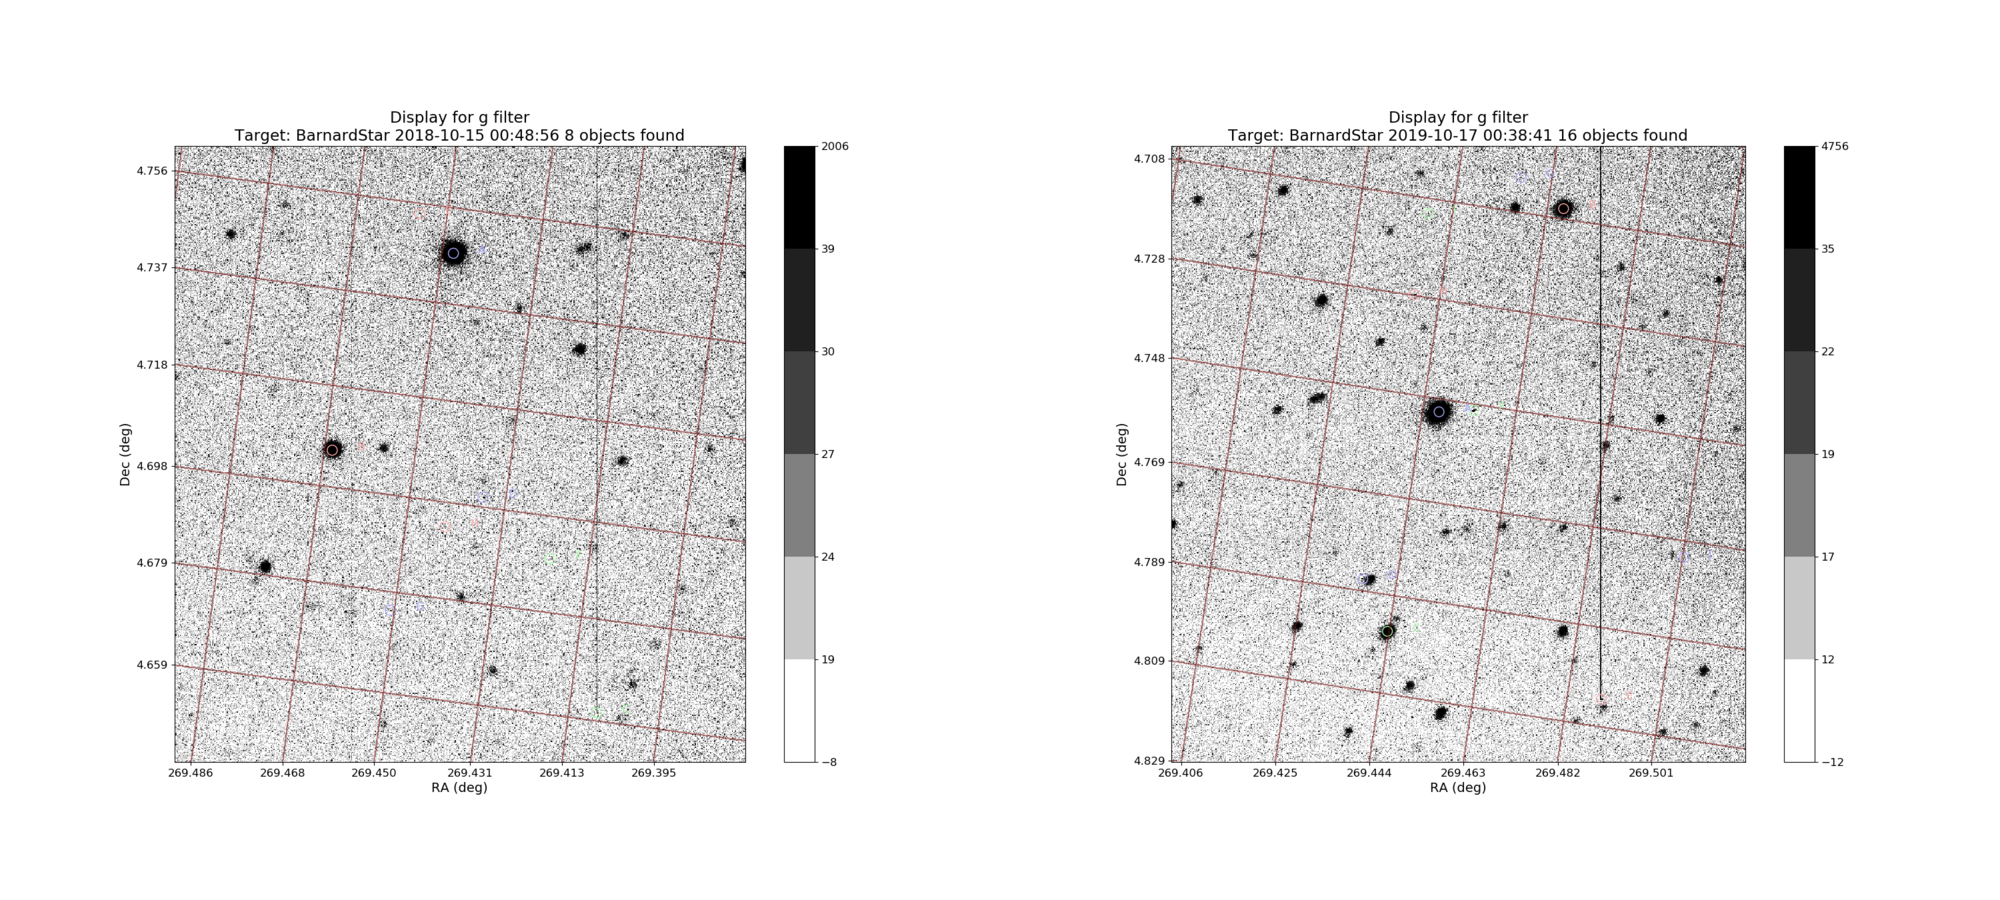
\includegraphics[scale=0.25]{images/yearapart.png} \\
\end{center}   
\caption{In this figure is illustrated two observations with the \texttt{g}
filter of \bstar, taken almost exactly a year apart showing that few
stars, and none sufficiently bright, are found in common between the two other
than the target.}
\protect\label{fig:yearapart}
\end{figure}

\clearpage
